\documentclass[11pt,addpoints,answers]{exam}
\usepackage[margin=1in]{geometry}
\usepackage{amsmath, amsfonts}
\usepackage{enumerate}
\usepackage{graphicx}
\usepackage{titling}
\usepackage{url}
\usepackage{xfrac}
\usepackage{geometry}
\usepackage{graphicx}
\usepackage{natbib}
\usepackage{amsmath}
\usepackage{amssymb}
\usepackage{amsthm}
\usepackage{paralist}
\usepackage{epstopdf}
\usepackage{tabularx}
\usepackage{longtable}
\usepackage{multirow}
\usepackage{multicol}
\usepackage[colorlinks=true,urlcolor=blue]{hyperref}
\usepackage{fancyvrb}
\usepackage{algorithm}
\usepackage{algorithmic}
\usepackage{float}
\usepackage{paralist}
\usepackage[svgnames]{xcolor}
\usepackage{enumerate}
\usepackage{array}
\usepackage{times}
\usepackage{url}
\usepackage{comment}
\usepackage{environ}
\usepackage{times}
\usepackage{textcomp}
\usepackage{caption}
\usepackage[colorlinks=true,urlcolor=blue]{hyperref}
\usepackage{listings}
\usepackage{parskip} % For NIPS style paragraphs.
\usepackage[compact]{titlesec} % Less whitespace around titles
\usepackage[inline]{enumitem} % For inline enumerate* and itemize*
\usepackage{datetime}
\usepackage{comment}
% \usepackage{minted}
\usepackage{lastpage}
\usepackage{color}
\usepackage{xcolor}
\usepackage{listings}
\usepackage{tikz}
\usetikzlibrary{shapes,decorations,bayesnet}
%\usepackage{framed}
\usepackage{graphicx}
\usepackage{booktabs}
\usepackage{cprotect}
\usepackage{xcolor}
\usepackage{verbatimbox}
\usepackage[many]{tcolorbox}
\usepackage{cancel}
\usepackage{wasysym}
\usepackage{mdframed}
\usepackage{subcaption}
\usetikzlibrary{shapes.geometric}

%%%%%%%%%%%%%%%%%%
% Begin Document %
%%%%%%%%%%%%%%%%%%


\begin{document}

\section*{}


\section*{START HERE: Instructions}

\textbf{Submitting your work:}

\begin{itemize}
\item \textbf{Deliverables:} Please submit all the \texttt{.py} files. Add all relevant plots and text answers in the boxes provided in this file. TO include plots you can simply modify the already provided latex code. Submit the compiled \texttt{.pdf} report as well.
\end{itemize}
\emph{NOTE: Partial points will be given for implementing parts of the homework even if you don't get the mentioned numbers as long as you include partial results in this pdf.}
\clearpage

\section{Image Captioning with Transformers (70 points)}



We will be implementing the different pieces of a Transformer decoder (\href{https://arxiv.org/pdf/1706.03762.pdf}{Transformers}), and train it for image captioning on a subset of the \href{https://cocodataset.org/#home}{COCO dataset}. 
\begin{itemize}
    \item \textbf{Setup:} Run the following command to extract COCO data, in the \texttt{transformer\_captioning/datasets} folder : \texttt{./get\_coco\_captioning.sh}
    %: \\ 
    % \texttt{get_coco_captioningsh}
\item \textbf{Question:} Follow the instructions in the \texttt{README.md} file in the \texttt{transformer\_captioning} folder to complete the implementation of the transformer decoder.
\item \textbf{Deliverables:} After implementing all parts, use run.py for training the full model. The code will log plots to \texttt{plots}. Extract plots and paste them into the appropriate section below. 

\item \textbf{Expected results:}
    These are expected training losses after 100 epochs. Do not change the seed in run.py.
    \begin{itemize}
        \item 2-heads, 2-layers, lr 1e-4: Final loss $\leq$ 1 
        \item 4-heads, 6-layers, lr 1e-4: Final loss $\leq$ 0.3 
        \item 4-heads, 6-layers, lr 1e-3: Final loss $\leq$ 0.05
    \end{itemize}
\end{itemize}

\begin{questions}
\question Paste training loss plots for each of the three hyper-param configs
\\
2-heads-2-layers-lr-1e-4: \textbf{TODO: fill in final train loss here.} \\
4-heads-6-layers-lr-1e-4: \textbf{TODO: fill in final train loss here.} \\
4-heads-6-layers-lr-1e-3: \textbf{TODO: fill in final train loss here.} 
\begin{figure}[H]
    \centering
    % TODO: put your plot here.
    \begin{subfigure}[b]{0.32\linewidth}
        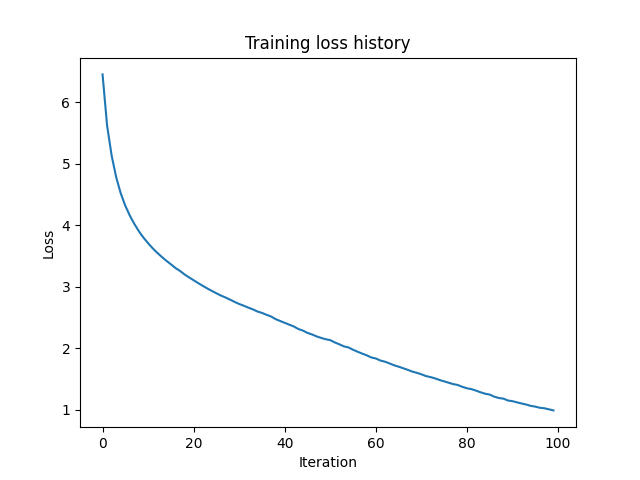
\includegraphics[width=\linewidth]{case1_loss_out.png}
        \caption{2-heads-2-layers-lre-4}
    \end{subfigure}
    \begin{subfigure}[b]{0.32\linewidth}
        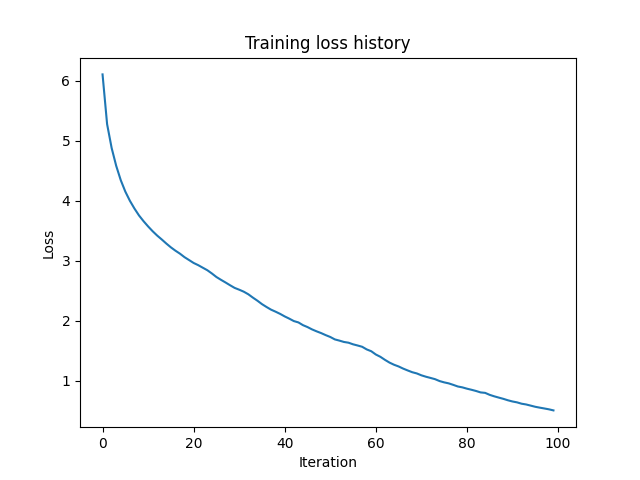
\includegraphics[width=\linewidth]{case2_loss_out.png}
        \caption{4-heads-6-layers-lre-4}
    \end{subfigure}
    \begin{subfigure}[b]{0.32\linewidth}
        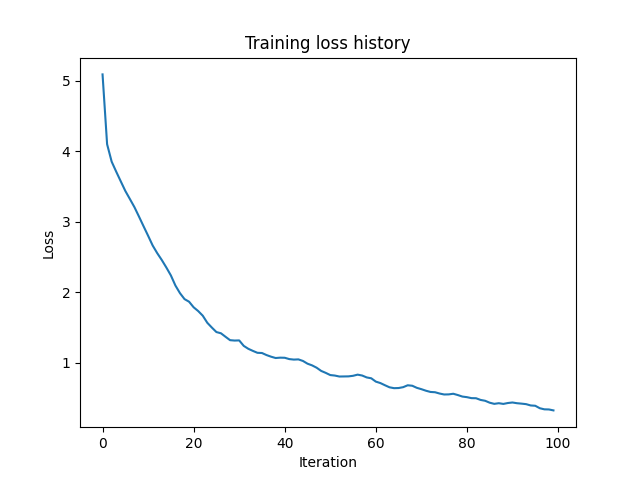
\includegraphics[width=\linewidth]{case3_loss_out.png}
        \caption{4-heads-6-layers-lre-3}
    \end{subfigure}
    
\end{figure}
\question Paste any three generated captioning samples from the training set with the three different settings. The provided code creates these plots at the end of training.
\\
\begin{figure}[H]
    \centering
    \begin{subfigure}[b]{0.32\linewidth}
        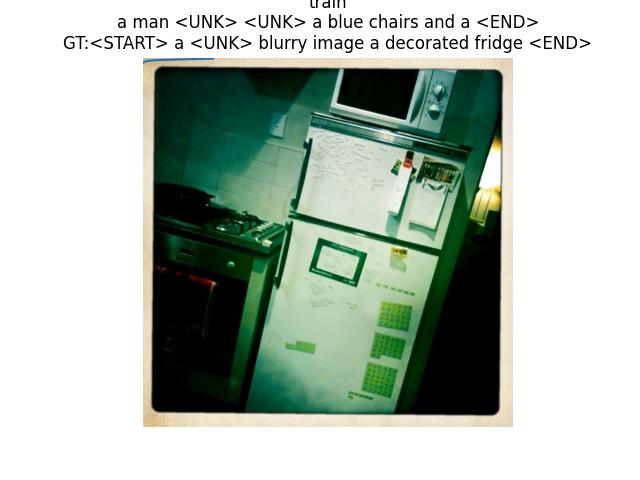
\includegraphics[width=\linewidth]{case1_train_3.png}
        \caption{Sample1: 2-heads-2-layers-lre-4}
    \end{subfigure}
    \begin{subfigure}[b]{0.32\linewidth}
        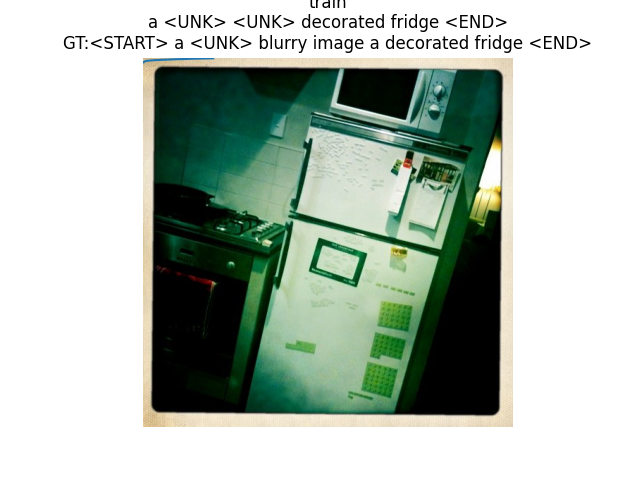
\includegraphics[width=\linewidth]{case2_train_3.png}
        \caption{Sample2:4-heads-6-layers-lre-4}
    \end{subfigure}
    \begin{subfigure}[b]{0.32\linewidth}
        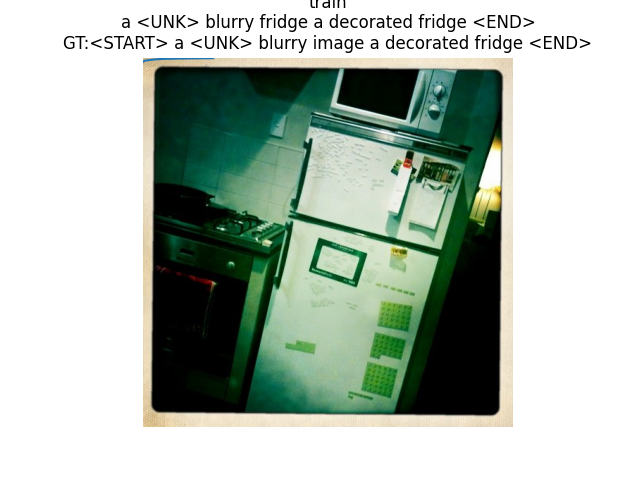
\includegraphics[width=\linewidth]{case3_train_3.png}
        \caption{Sample3:4-heads-6-layers-lre-3}
    \end{subfigure}
\end{figure}

\item Based on the observations of the three different settings, What would you change in the training procedure to get better validation performance? Why tweaking these hyper-parameters will lead to better performances?

\begin{solution}
% YOU ANSWER HERE
\begin{itemize}
    \item {Learning Rate}
    
    Learning rate describes the step size when getting the mininum of the loss function.If the learning rate is too low the training process will be slow and may get stuck in a local minimum.And if it is too high, it may cause the model to oscillate around,as the loss history picture of model with learing rate = 1e-3  shows that the loss is oscillating when converge to the mininum.

    \item{number of layers}

    A big number of layer can improve the Representational Capacity of the model, and may do more complicated works,and as a result it will also make the model more complex,which will raise the trainging time and training difficulty,and it may require more computation resource and trainging data.

    \item{number of attention heads}

    More attention heads lead to a better information acquisition from the trainging data,but will also consume more computaton resource because every attention head need to calculate its attention function and generate more temperorary results.

    \item{Optimizer}

    The use of different optimizers have various impacts on the trainging speed and performance of the model

    \item{Batch size}

    Larger batch sizes typically provide more stable gradient estimates,and may improve the model performance.However, if the batch size if too large it may lead to overfitting.
    
\end{itemize}


\end{solution}


\end{questions}
\clearpage

\section{Classification with Vision Transformers (30 points)}



We will use the transformer you implemented in the previous part to implement a Vision Transformer (\href{https://arxiv.org/abs/2010.11929}{ViT}), for classification on CIFAR10. 

\begin{itemize}
    \item \textbf{Question:} Follow the instructions in the \texttt{README.md} file in the \texttt{vit\_classification} folder. You are encouraged to resuse code from the previous question. 
    \item \textbf{Deliverables:} Run training using \texttt{run.py} for training the full model. The code will log plots \texttt{acc\_out.png} (train and test accuracy) and \texttt{loss\_out.png} (train loss). 
    \item \textbf{Expected Results:} After 100 epochs, test accuracy should be $\geq 65\%$, train accuracy should be $\approx 100\%$, and training loss $\leq 0.3$. 
\end{itemize}

\begin{figure}[H]
    \centering
    \begin{subfigure}[b]{0.32\linewidth}
        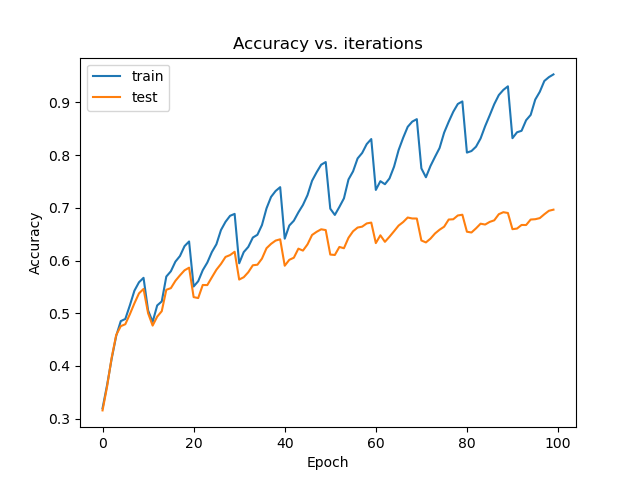
\includegraphics[width=\linewidth]{acc_out.png}
        \caption{Train/test accuracy}
    \end{subfigure}
    \begin{subfigure}[b]{0.32\linewidth}
        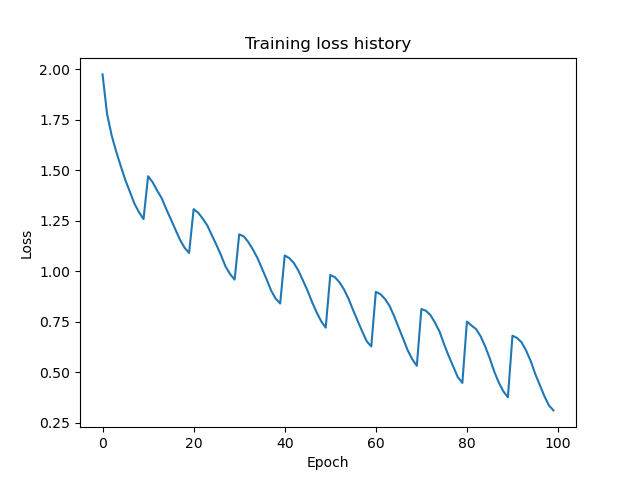
\includegraphics[width=\linewidth]{loss_out.png}
        \caption{Training loss}
    \end{subfigure}
\end{figure}

\clearpage

\textbf{Collaboration Survey} Please answer the following:

\begin{enumerate}
    \item Did you receive any help whatsoever from anyone in solving this assignment?
    \begin{checkboxes}
     \choice Yes
     \CorrectChoice No
    \end{checkboxes}
    \begin{itemize}
        \item If you answered `Yes', give full details:
        \item (e.g. “Jane Doe explained to me what is asked in Question 3.4”)
    \end{itemize}

    \begin{tcolorbox}[fit,height=3cm,blank, borderline={1pt}{-2pt},nobeforeafter]
    %Input your solution here.  Do not change any of the specifications of this solution box.
    \end{tcolorbox}

    \item Did you give any help whatsoever to anyone in solving this assignment?
    \begin{checkboxes}
     \choice Yes
     \CorrectChoice No\
    \end{checkboxes}
    \begin{itemize}
        \item If you answered `Yes', give full details:
        \item (e.g. “I pointed Joe Smith to section 2.3 since he didn’t know how to proceed with Question 2”)
    \end{itemize}

    \begin{tcolorbox}[fit,height=3cm,blank, borderline={1pt}{-2pt},nobeforeafter]
    %Input your solution here.  Do not change any of the specifications of this solution box.
    \end{tcolorbox}

    \item Note that copying code or writeup even from a collaborator or anywhere on the internet violates the \href{hhttps://www.cmu.edu/policies/student-and-student-life/academic-integrity.html}{Academic Integrity Code of Conduct}.
\end{enumerate}

\end{document}